\chapter{Evolución de la enfermedad en un entorno controlado}

A continuación nos situaremos en un escenario un poco más realista. Supongamos que se descubre el inicio de un brote de gripa en el hospital de un pueblo con 49 personas y deseamos analizar el comportamiento de la enfermedad para establecer medidas de control para variaciones futuras de la misma gripa.

En el pueblo podemos identificar cinco lugares diferentes en donde las células interactúan entre sí: La escuela, las oficinas, el mercado, el hospital y las viviendas de cada persona. Asumiremos que en la población se realizó un censo y tenemos acceso a las edades de cada individuo, su lugar de trabajo (o donde pasan la mayor parte del tiempo) y las personas con las que viven. Distribuyéndose de la siguiente manera:

\begin{itemize}
    \item \textbf{Escuela (E):} Se sabe que en el pueblo hay 9 niños y 2 profesores.
    \item \textbf{Oficinas (O):} Cuenta con un personal de 16 individuos.
    \item \textbf{Mercado (M):} Se identificaron 8 trabajadores.
    \item \textbf{Hospital (H):} Entre doctores, enfermeros y pacientes se identifica una cantidad de 14 individuos.
\end{itemize}

Supondremos que todos los niños del pueblo son hijos únicos y que las viviendas con tres individuos cuentan con al menos un niño. Además de esto y de acuerdo con la información anterior supondremos que en el pueblo la población vive en uno de tres tipos de vivienda: la vivienda C1 en donde vive una sola persona y que se asume además que es un adulto; las viviendas C2 en donde viven dos individuos, ya sean dos adultos o un adulto y un niño; y por último las viviendas C3, en donde viven 3 personas.

\begin{figure}[h]\label{fig:edadesYOcupaciones}
  \centering
    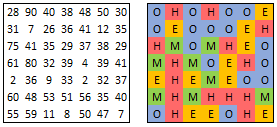
\includegraphics[width=0.3525\textwidth]{Imagenes/edadesYOcupaciones.PNG}
    \caption{Edades y ocupaciones en el pueblo.}
\end{figure}

De acuerdo con lo mencionado en el capítulo anterior, debemos establecer los grados de impacto de acuerdo con la manera en la que se distribuye nuestra población. En nuestro caso asumiremos que las personas que viven juntas tienen una grado de impacto cero entre ellas, que con los que tienen contacto en el lugar de ocupación tienen un grado de impacto igual a uno y que con las demás células tienen grado de impacto dos. De ese modo, si organizamos a la población sobre una malla identificando sus edades, ocupaciones y vecindades obtendremos algo como lo que se ve en la siguiente figura:

\begin{figure}[h]\label{fig:edadesYOcupaciones}
  \centering
    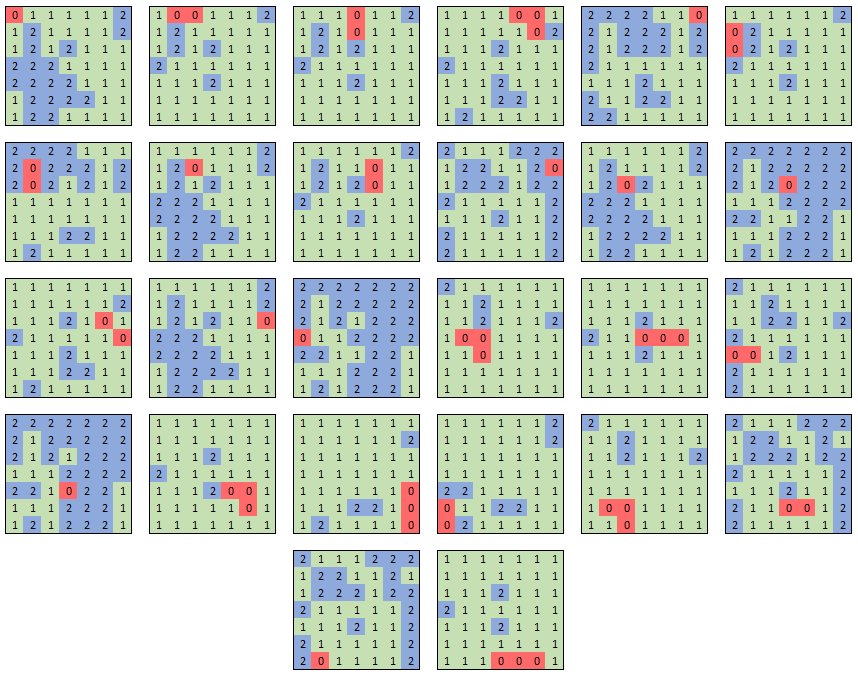
\includegraphics[width=1\textwidth]{Imagenes/vecindadesCap4.PNG}
    \caption{Grados de impacto.}
\end{figure}

En el caso de la enfermedad, supondremos que dura en promedio 5 días, por lo que tomaremos $\alpha=\frac{1}{5}=0.2$ y por otro lado tomaremos una tasa de infección $\beta=0.3$, supondremos unas tasas de natalidad y de mortalidad iguales a 0.02 y 0.005 respectivamente y finalmente, asumiremos que de brotes de gripa anteriores se tiene que las tasas de letalidad de la enfermedad son:

\begin{table}[h]
\begin{center}
\begin{tabular}{| c | c |}
\hline
Rango de edades & Tasas \\ \hline
1 - 15 & 0.005 \\
16 - 48 & 0.01 \\
49 - 55 & 0.1 \\
56+ & 0.25 \\\hline
\end{tabular}
\caption{Tasas estimadas de letalidad de la gripa en el pueblo}
\end{center}
\end{table}

Analizaremos el comportamiento de la enfermedad en un periodo de 30 días tomando diferentes tasas de impacto. Esto nos brindará una visión de las implicaciones que pueden llegar a tener las relaciones más cercanas con individuos fuera de la vecindad mínimal en el evento donde se propaga alguna enfermedad.